% Compile with XeLaTeX (Overleaf: Menu -> Compiler -> XeLaTeX).
% v2 reframe: the paper leads with convergence, invariants, and tail exploration;
% block detail and equations live in Appendix A. ~8K words.
\documentclass[a4paper,fleqn]{cas-sc}

\usepackage[numbers,sort&compress]{natbib}
\usepackage{subcaption}
\usepackage{tabularx}
\usepackage{graphicx}
\graphicspath{{figures/}}
\usepackage{xcolor, soul}
% cas-common.sty defines L as a non-wrapping fill column; the tables need a wrapping one.
\newcolumntype{L}{>{\raggedright\arraybackslash}X}

% First-page footer. Deliberately names no journal: this version has not been submitted
% anywhere, and printing a target on a preprint that ships in a public archive would read
% as a submission that has not happened.
\ExplSyntaxOn
\cs_set:Npn \__first_footerline:
{
  \group_begin:
  \small \sffamily
  \ifnum\theblind>0\relax \else \__short_authors: :~ \fi
  { \rmfamily \itshape Preprint~ --~ not~ peer~ reviewed }
  \group_end:
}
\ExplSyntaxOff

\begin{document}
\let\WriteBookmarks\relax
\def\floatpagepagefraction{1}
\def\textpagefraction{.001}

\shorttitle{Integrated World Model}
\shortauthors{Sotiriadi~N. et~al.}

\title[mode = title]{An Integrated World Model for Strategic Planning and Scenario Analysis}
\author[1]{Nazar S.~Sotiriadi}[orcid=0009-0006-1116-896X]
\cormark[1]
\ead{sotiriadi.n.s@gmail.com}
\author[2]{Alexander N.~Krenke}[]
\author[1,3]{Andrei A. Osiptsov}[]
\affiliation[1]{organization={JSC Sberbank of Russia}, addressline={Kutuzovsky avenue, 32}, city={Moscow}, citysep={}, postcode = {121170}, country={Russian Federation}}
\affiliation[2]{organization={Institute of Geography, Russian Academy of Sciences}, addressline={Staromonetny lane, 29, bld. 4}, city={Moscow}, citysep={}, postcode = {119017}, country={Russian Federation}}
\affiliation[3]{organization={Skolkovo Institute of Science and Technology (Skoltech)}, addressline={Bolshoy Boulevard 30, bld. 1}, city={Moscow}, citysep={}, postcode = {121205}, country={Russian Federation}}

\date{\today}

\maketitle

\begin{center}
\fbox{\parbox{0.92\linewidth}{\small\textbf{Preprint.} This is an unrefereed preprint. It has
not been peer reviewed and is not published in any journal. Numbers, claims and figures may
change in revision. The model version it describes, together with the validation evidence
behind every claim made here, is archived at \url{https://github.com/Theclimateguy/GIM}
(branch \texttt{GIM20.1}) and on Zenodo; please cite the software record rather than this
document.}}
\end{center}
\medskip

\begin{abstract}
\noindent
\textbf{Motivation.} Coupling the economy, climate, society, and geopolitics in one closed
simulator is easy to attempt and hard to sustain: such loops generically diverge, stick in
absorbing states, or must be damped into triviality. We present a global integrated model (GIM)
--- 57 country agents, seven coupled domains, an annual deterministic loop --- built as an
explicit encoding of invariants (conservation laws, accounting identities, slow empirical
regularities) with calibrated restoring forces.
\textbf{Methods.} Stability is measured, not asserted: numerical linearization of the annual
map, twin runs from perturbed initial states, and a 500-member history-matched parametric
ensemble; anchoring uses a 2015--2023 retrospective fit against output, emissions, temperature
and resource prices, a free-running out-of-sample window at 2020--2023, and an
input-vintage-robust conflict ranking.
\textbf{Results.} The spectral radius is $1.036$--$1.100$ over some thirty above-unity modes
whose mass sits mainly on economic coordinates (debt, unemployment, inflation), while the
climate subspace carries none of it and economic and climate perturbations contract ($0.975$ and
$0.970$ per year); the parametric, shock-inclusive fan grows near-linearly to $\pm10.8\,\%$ of
median world product at thirty years. In-sample errors are $0.60$ trillion USD (country-level
output), $0.94$ Gt CO$_2$, $0.145\,^{\circ}$C; on the untouched 2020--2023 window they are
$0.77$, $0.72$, $0.13$. Resource prices are scored against observed commodity indices and beat a
flat-price null on all three. Conflict ranking reaches AUC $0.739$ (1990--2023) and $0.84$ with
pre-2000 inputs on 2000--2023 --- though its single dominant input scores $0.777$ alone, so the
composite adds nothing detectable over it. A game layer adversarially samples the tails:
$1{,}002$ scripted runs (23.5\,\% survival) and 200 completed human runs of 401 started
(28.5\,\% of completers) map how a managed world fails, and exposed two structural degeneracies
invisible to retrospective validation.
\textbf{Conclusion.} GIM is a bounded, anchored, responsive exploration instrument --- not a
forecast engine.

\medskip
\noindent\textbf{Keywords:} integrated assessment model, world simulation, stability, invariants, uncertainty quantification, serious games, weak signals.
\end{abstract}

\section{Introduction: the hard part is staying together}

Strategic planning and systemic-risk work need a tool in which climatic, economic, and
socio-political processes are considered jointly: the paths that matter --- warming to crop
yields to prices to social tension to instability --- cross domain boundaries that sectoral
models do not \citep{nordhaus2017,riahi2017}. That gap is well known. What is less discussed is
why it persists. Coupling the domains is not conceptually difficult; the difficulty is that a
\emph{closed} loop through economy, climate, society, and politics is a high-dimensional
nonlinear dynamical system, and such systems do not stay plausible by default
\citep{may1972,sterman2000}. In our experience they fail in a small number of characteristic
ways: variables run to a bound and stick (absorbing states), accounting errors compound into
runaway growth, latent variables drift to structural attractors that no policy can move, or ---
the opposite failure --- every feedback is damped until the simulator reproduces a trend line
and nothing else. A world model earns its keep in the space between these failures: bounded for
decades, yet still able to generate crises, cascades, and lags.

This paper reports a model built and validated to live in that space, and reframes what we
consider its main result. The Global Integrated Model (GIM) advances 57 country agents (the 50
largest economies plus seven regional aggregates that conserve world totals) through an annual
deterministic loop spanning the economy and prices, climate and the carbon cycle, natural
resources, society and politics, interstate relations, and discrete crises with
stock-flow-consistent finance. Its headline property is not the breadth of coverage but the
combination of three measured behaviours: (i)~\emph{convergence} --- thirty-year trajectories
are bounded, insensitive to small initial-state perturbations, and their ensemble uncertainty
grows near-linearly rather than exponentially (Section~\ref{sec:stability}); (ii)~\emph{anchor}
--- the same configuration reproduces 2015--2023 history in-sample, is scored free-running on an
untouched 2020--2023 window, and carries out-of-sample skill where structure matters
(Section~\ref{sec:valid});
(iii)~\emph{responsiveness} --- the loop produces structured dynamics (lagged social channels,
threshold-stepped sovereign cascades, cross-block synchrony of failures) whose shapes go beyond the coded
terms they build on (Section~\ref{sec:emergent}).

The stance behind (i) is methodological and we state it up front: the deterministic core is an
explicit hypothesis about \emph{invariants} --- the conservation laws, accounting identities,
and slowly-varying empirical regularities that we take to govern nature and society
(Section~\ref{sec:invariants}). Determinism is then a feature, not a naivety: the core computes
what follows \emph{if} those invariants hold, and all uncertainty is carried by ensembles over
the invariants' strengths. On top of this core sits an instrument layer --- history-matched
ensembles, weak-signal detectors, and a decision game that operates as an adversarial sampler
of the tails, including live outcome telemetry from external players
(Section~\ref{sec:instrument}). The model does not claim predictive foresight; at horizons beyond two--three years,
professional growth forecasts lose to a naive mean-growth benchmark in roughly half of countries
\citep{celasun2021}, and we hold this model to the same bar (Section~\ref{sec:valid}).

Relative to the integrated-assessment and world-modeling traditions --- DICE/RICE
\citep{nordhaus2017,nordhausyang1996} and FUND \citep{anthoff2013} (welfare optimisation), GCAM
\citep{calvin2019} and MESSAGEix \citep{huppmann2019} (energy-system equilibrium), E3ME
\citep{mercure2018} (econometric simulation), T21/iSDG \citep{barney2002} (single-country system
dynamics), World3 \citep{meadows1972} (global aggregates) --- GIM's distinction is that it closes
the loop through society, geopolitics, and discrete crises at country resolution and then
\emph{demonstrates} that the closed loop is stable, anchored, and non-trivial. A controlled
benchmark quantifying what the closed loop sees and sectoral models structurally cannot is kept
in Appendix~\ref{app:benchmark}; the model specification (functional forms, parameters) is
compressed into Appendix~\ref{app:spec}.

A comprehensive review by Keppo et al.~\citep{keppo2021} identifies six persistent critiques of
IAMs: heterogeneous actors, technology diffusion, capital markets, energy--economy feedbacks,
policy scenarios, and model interpretation. GIM directly addresses several of these: it embeds
heterogeneous country agents with bilateral relations, includes an endogenous R\&D-stock
mechanism and trade-driven diffusion, implements stock-flow-consistent finance with sovereign
debt and crisis dynamics, and couples energy prices, inflation, and social tension in a single
loop. The remaining critiques (policy differentiation and result interpretation) are addressed
in Sections~\ref{sec:emergent} and~\ref{sec:instrument}.

\section{The invariant view}
\label{sec:invariants}

Every long-horizon simulator embodies assumptions; ours are organized deliberately into three
classes of invariants, in descending order of confidence, plus a fourth element that keeps the
loop near them.

\textbf{Physical conservation.} Carbon is conserved: each year's emissions are partitioned into
the four IPCC AR6 impulse-response pools and decay on fixed timescales; atmospheric stock,
radiative forcing, and the two-reservoir surface--ocean heat balance follow standard
reduced-complexity climate physics \citep{joos2013,geoffroy2013,ipcc_ar6_wg1}, the same
architecture as the FaIR and MAGICC emulators \citep{smith2018fair,meinshausen2011}, with the
emission record anchored to the Global Carbon Budget \citep{friedlingstein2023}. The block reproduces both
assessed constants an AR6-consistent emulator must match: equilibrium sensitivity
$3.0\,^{\circ}$C and transient response $1.79\,^{\circ}$C (AR6 best estimate 1.8).

\textbf{Accounting identities.} Money and goods cannot appear from nowhere: the financial side
is stock-flow consistent (every loan creates a matching deposit; the money stock is identically
deposits and loans) \citep{godley2007}; government budgets close; bilateral trade settles in
reserves and world net exports sum to zero by an enforced invariant; excessive borrowing raises
the cost of credit --- a financial accelerator \citep{bernanke1999}. These identities are
checked at runtime, not assumed.

\textbf{Empirical regularities as slow variables.} Between hard conservation and free
parameters sits a class of relationships that are not laws but have been stable across decades
and countries, and we treat them as invariants with priors on their strength: trade follows a
gravity law in distance \citep{headmayer2014}; unemployment follows Okun's law and inflation a
flat post-1990 Phillips curve with a weak quantity-theory term; poorer economies converge
toward the frontier at a $\beta$-convergence rate validated against the cross-section; the
public's response to unemployment and inflation follows the two-to-one misery-index ratio;
war sizes follow a power law \citep{richardson1948,clauset2009}; institutions are anchored to
governance indices, culture to the Hofstede dimensions \citep{kaufmann2011,hofstede2010}.
Monetary policy follows country-level Taylor rules \citep{taylor1993}. Where a regularity
failed the data --- a classic Richardson arms-race term, rejected at $p=0.74$ on the 1995--2024
military-expenditure panel --- it was left out and the observed state variable used instead.

\textbf{Equilibrium anchors and restoring forces.} Invariants alone do not prevent drift;
bounded behaviour comes from explicit restoring terms whose strengths are calibrated, not
hidden: resource prices mean-revert in log space toward reference levels; production is
normalized so each country's base point is exactly reproduced (a normalized-CES discipline that
pins levels while leaving substitution free); trust and tension carry anchor terms; crisis
states have exit conditions. Section~\ref{sec:stability} shows what these forces achieve and
Section~\ref{sec:instrument} how two missing anchors were found the hard way. The full
functional forms and the 33 literature-grounded priors are in Appendix~\ref{app:spec}.

Determinism, in this view, is the point: the core is a reproducible mapping from an invariant
set to trajectories. Following \citet{oreskes1994}, we do not claim the model is verified truth
--- we claim it is a confirmed, auditable encoding of stated assumptions, evaluated by whether
its trajectories stay within the envelope of observed history and whether its failures are
informative.

\section{Architecture: one closed loop}
\label{sec:arch}

One model step is one year; blocks update in fixed order and the year's outputs are the next
year's inputs (Fig.~\ref{fig:arch}). The economy is the hub: output comes from capital, labour,
and energy through a nested CES function; markets clear by price; inflation, unemployment,
budgets, debt, and bilateral trade are tracked per country. Output emits CO$_2$ (declining
structural intensity); emissions accumulate in the carbon pools; warming returns as a quadratic
output damage. Resource stocks and world prices couple scarcity into inflation. Society tracks
trust, tension, inequality, legitimacy, and protest pressure, all responding to economic stress
with explicit coefficients; politics converts legitimacy into a policy-space multiplier;
geopolitics carries relations, alliances, sanctions, and a CINC-style capability index
\citep{singer1972} grounded in SIPRI expenditure. The 2023 base-year world product of the 57
agents is ${\approx}107$ trillion USD, so the thirty-year baseline median of $241$ implies
${\approx}2.7\,\%$ median annual growth. Discrete crises --- debt, currency, regime collapse --- fire on threshold
crossings, apply audited state changes (a 40\,\% debt write-down, output and trust hits), and
have exit rules. Conflict, unrest, and climate risk spill over to geographic neighbours; a
shock in any block propagates along realistic pathways: carbon price to energy cost to
emissions; hardship to tension to savings to crisis risk; crisis to trade partners. The
feedback signs matter more than the functional detail (which is deferred to
Appendix~\ref{app:spec}): the loop mixes amplifying channels (financial accelerator, crisis
contagion, tension--trust spiral) with the restoring forces of Section~\ref{sec:invariants},
and the balance between them is what the next section measures.

\begin{figure}[t]
\centering
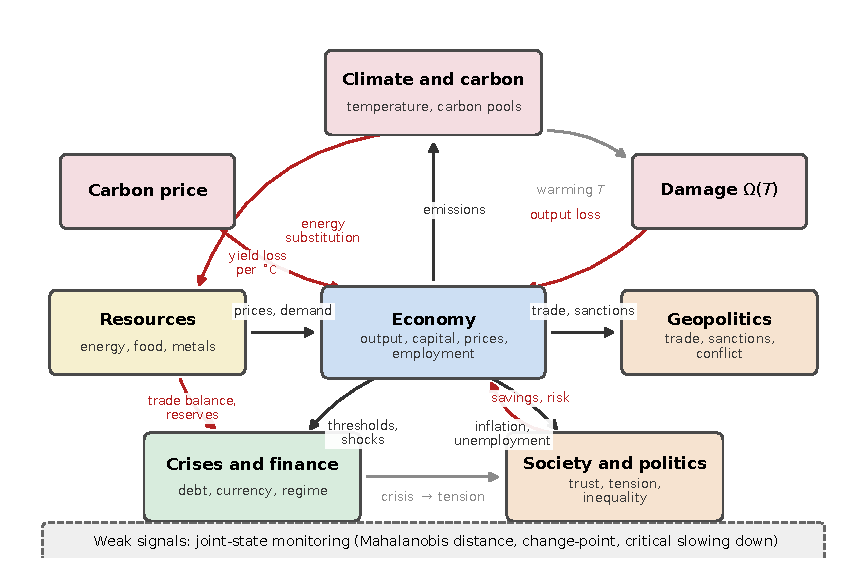
\includegraphics[width=\linewidth]{fig1_architecture.pdf}
\caption{The closed loop. Economy at the hub, physical blocks above it and human blocks below.
Dark arrows are direct effects, red arrows are the channels that reduce output, savings or
supply --- climate damage, energy substitution, the per-degree yield loss on crops, and the
resource trade balance that drives reserves and the sovereign channel. The climate loop
(emissions $\to$ warming $\to$ damage $\to$ output) is complemented by carbon-price, resource,
socio-political, geopolitical and discrete-crisis channels. The bottom layer monitors the joint
state for weak signals.}
\label{fig:arch}
\end{figure}

\section{What keeps it together: stability, measured}
\label{sec:stability}

Convergence claims are cheap; we support ours with three quantitative diagnostics plus the
engineering discipline that maintains them. All runs below use the deterministic core (simple
background policy, extreme events off); the harness is
\texttt{scripts/run\_stability\_analysis.py}.

\textbf{Spectral radius of the one-year map.} We linearize the full annual map
$x_{t+1}=F(x_t)$ numerically (central differences) around the baseline trajectory in a
408-dimensional state space --- seven variables per agent (output, capital, debt, unemployment,
inflation, trust, tension) plus the nine global coordinates (surface and ocean temperature, four
carbon pools, three resource prices) --- at three points along the run. Eigenvalues are computed
on $D^{-1}JD$ with $D$ the diagonal of trajectory-mean coordinate scales --- a similarity
transform that leaves the spectrum unchanged and only conditions the eigenvector readout. The
spectral radius is $\rho(J)=1.036$, $1.100$, $1.041$ at 2026, 2036, 2046, over $36$, $35$ and
$31$ above-unity modes (Fig.~\ref{fig:stability}a).

Two properties of that spectrum deserve emphasis, because together they set what a stability
claim about a model of this kind can assert.

The first is a specification requirement rather than a result. A bounded state variable with no
restoring force of its own carries a unit eigenvalue by construction, so it will place modes on
the unit circle whatever the coupling does, and a spectral radius computed over it measures the
omission rather than the loop. Institutional trust is the case in point: it is bounded in
$[0,1]$, and its drivers --- inequality, unemployment, inflation --- have to enter as deviations
from a reference rather than as levels, or an agent at constant and entirely ordinary conditions
loses trust every year without limit. The deviation form removes that drift; it does not remove
the unit root, since a walk without drift still sits at $|\lambda|=1$. GIM therefore also gives
trust the weak mean reversion its resource prices already carry (Appendix~\ref{app:spec}), and
we report the spectrum of the resulting map. The diagnostic value of the exercise is that it
separates a deficiency of specification from a property of the coupled system, which a spectral
radius on its own cannot do.

The second is the result. Modes above unity remain --- the loop does not contract everywhere ---
but their mass sits mainly on \emph{economic} coordinates: public debt compounding near the
effective interest rate, unemployment, inflation, carrying $0.57$, $0.65$ and $0.78$ of the
loading at the three linearization points against the social block's $0.43$, $0.35$ and $0.22$.
The climate coordinates carry none of it: across every configuration we examined, with and
without the trust anchor, the above-unity mass on temperature, ocean heat and the carbon pools
is $0.00$. Contraction of the economic--climate subspace is thus the firm part of the finding,
and the residual asymmetry between physical and social directions is real but modest. We report
it as a property of this model at this calibration, not as a general feature of coupled world
models.

\textbf{Perturbation contraction.} The trajectory-level counterpart: twin runs from
$\varepsilon$-perturbed initial states, gaps measured as dimensionless relative differences in
world product. A $+0.1\,\%$ shock to United States output (a vector with essentially no
projection on the socio-fiscal modes above) produces a relative gap of $2.6\times10^{-4}$ after
one year that \emph{contracts} to $1.2\times10^{-4}$ by year 30 --- an empirical factor of
$0.975$ per year; a $+0.01\,^{\circ}$C temperature perturbation decays at $0.970$ per year.
Nearby trajectories converge in the economic--climate subspace --- the opposite of chaotic
divergence (Fig.~\ref{fig:stability}b). The one persistent direction is the one the spectrum
names: raising every country's tension by $0.01$ leaves output almost untouched for a decade and
then amplifies as crisis triggers engage, reaching a $2.5\,\%$ world-product gap by 2053. The spectrum, the twin runs, and the fan below
therefore tell one story rather than three: contraction in the physical--economic directions,
slow amplification confined to the socio-fiscal subspace. We report the asymmetry as a
substantive property, not a defect --- and it quantifies the limitation that socio-political
initial-state error does not wash out (Section~\ref{sec:limits}).

\begin{figure}[t]
\centering
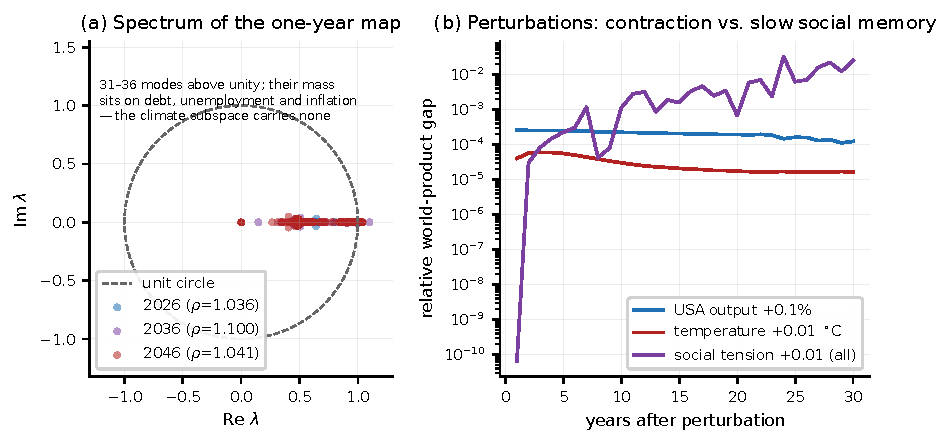
\includegraphics[width=\linewidth]{fig12_stability.pdf}
\caption{Local stability of the annual map. \emph{(a)}~Eigenvalues of the (similarity-)
normalized Jacobian (408-dimensional state) at three linearization years. The spectrum lies on
and inside the unit circle apart from $31$--$36$ modes just outside it, giving
$\rho(J)=1.036$, $1.100$, $1.041$; their eigenvector mass sits mainly on economic coordinates
--- public debt, unemployment, inflation --- carrying $0.57$--$0.78$ against the social block's
$0.22$--$0.43$, while the climate coordinates carry none of it. \emph{(b)}~Twin-run response
(relative world-product gap): output and temperature perturbations contract at $0.975$ and
$0.970$ per year, while a broad social-tension perturbation persists and amplifies --- the
model's one long-memory direction.}
\label{fig:stability}
\end{figure}

\textbf{Bounded, near-linear uncertainty growth.} A 500-member ensemble drawing the 33 key
priors from their history-matched ranges --- with the discrete-crisis machinery \emph{active}
(the members average one to three sovereign crises by 2053) --- runs the full 30 years without a
member diverging or saturating (Fig.~\ref{fig:ens30}). This is a \emph{parametric, conditional}
fan, not a forecast interval: members share the initial state, so much of its near-linear growth
is each member following its own prior-drawn trend, and non-divergence is partly by construction
since implausible corners were pruned by history matching. What the fan does bound is the
amplification rate: the world-product half-width grows from $\pm1.7\,\%$ of median at year 5 to
$\pm4.0\,\%$ at 10 and $\pm10.8\,\%$ at 30 (all 5--95th half-widths), an average exponential
rate below $0.08$\,yr$^{-1}$ with concave shape after year 10 --- any local instability
compounding materially faster than the socio-fiscal modes of the spectrum would bend this curve
upward, and none does. Two non-trending observables make the point without the trend caveat:
the mean-tension fan stays narrow and sub-linear (5--95th width $0.011$ at year 5, $0.026$ at
30, i.e.\ $2$--$5\,\%$ of its level), and the temperature fan widens only from $0.72$ to
$1.10\,^{\circ}$C between years 5 and 30 (full widths; the climate-sensitivity prior expresses
itself early). Median 2053 world product is $241$ trillion USD (5--95th: $215$--$270$) at
$+1.94\,^{\circ}$C ($1.39$--$2.49$); for calibration of scale, a single structural choice ---
renormalising production to constant returns --- moves 2100 world product by $7$--$9\,\%$, of
the same order as this whole parametric fan.

\textbf{The discipline that preserves this.} Stability is a maintained property, not a lucky
draw. Every change to the core faces pinned golden backtests (bit-identical or explicitly
recalibrated); calibration data are checksum-bound; every optional mechanism is a switch, off
by default unless anchored by evidence; and the invariants of Section~\ref{sec:invariants} are
runtime-checked. Two failures that this discipline did \emph{not} catch --- because they lived
outside the historical window --- were caught by the game layer
(Section~\ref{sec:instrument}); both fixes shipped as anchors of exactly the
Section~\ref{sec:invariants} type, with the historical backtests unchanged to the bit. One
caveat qualifies all of this: convergence here is
engineered and measured, not proven --- anchors strong enough to stabilize can in principle
mask real-world instabilities, which is why their strengths carry priors and the tails are
explored deliberately (Section~\ref{sec:instrument}).

\begin{figure}[t]
\centering
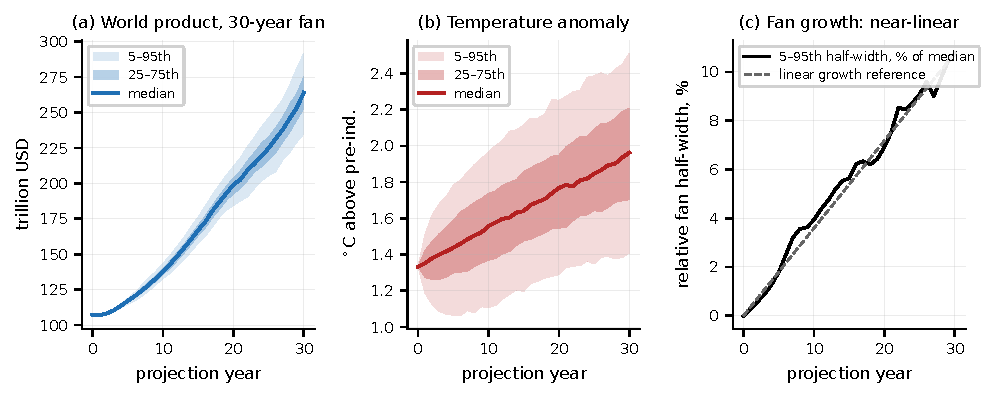
\includegraphics[width=\linewidth]{fig11_ensemble30.pdf}
\caption{Thirty-year boundedness evidence (500-member parametric ensemble, shared initial
state, discrete crises active). \emph{(a)}~World product fan: all members bounded, median
$264$T at 2053, 5--95th $235$--$292$T. \emph{(b)}~Temperature fan: full 5--95th width grows
$0.72\to1.10\,^{\circ}$C between years 5 and 30, median $1.96\,^{\circ}$C at 2053.
\emph{(c)}~Relative 5--95th half-width of world product reaches $10.8\,\%$ of the median at
thirty years and tracks a linear reference --- parametric uncertainty accumulates, with no
super-exponential bending.}
\label{fig:ens30}
\end{figure}

\section{Is it anchored? Validation against history}
\label{sec:valid}

A stable simulator can still be stably wrong; the second requirement is anchor to observation.
All retrospective runs are \emph{free-running}: initialized once from the 2015 state and never
re-anchored to observations, so errors are multi-year trajectory errors, not one-step-ahead
errors. The output metric is the RMSE over country-year pairs (20 largest economies), reported
in trillion USD; emissions and temperature are world-series RMSEs. The economic and climate
blocks are calibrated by history matching --- ruling out parameter regions whose implausibility
$I_o(\theta)=\mathrm{RMSE}_o(\theta)/\mathrm{tol}_o$ exceeds the three-sigma cut, a standard
approach for expensive simulators \citep{williamson2013} --- on the 2015--2023 world series;
the machinery is specified in Appendix~\ref{app:spec}. Because those metrics are in-sample by
construction, predictive adequacy is measured separately by a \emph{free-running temporal
out-of-sample test}: the model is initialized once, never re-anchored, and scored on 2020--2023,
a window that enters no calibration anywhere (\texttt{scripts/run\_holdout\_validation.py}).
We name the test for what confers its out-of-sample status --- that the window is used nowhere
--- rather than for the constraint step, because at these tolerances the constraint step confers
nothing. Re-running history matching through 2019 and freezing the retained region would be the
natural way to construct such a test, but the 2015--2019 window rules out no draw at all, so the
frozen region coincides with the prior box and the exercise reduces to running the same
configuration forward.

That the cut does not bind is worth quantifying rather than noting in passing, since it governs
how the calibration stage should be described. Over 600 draws from the prior box the maximum implausibility anywhere is $1.69$ against a cut at
$3.0$, with a median of $0.665$; the per-output tolerances are loose by a consistent factor of
about five, and world output spans only $I=0.594$--$0.619$ across the entire box, meaning the
window does not identify the economic parameters at all. History matching here is therefore a
\emph{ranking}, not a filter --- and as a ranking it works: per-output implausibility predicts
its own out-of-sample error at $\rho=0.90$--$0.95$. The usual $\max_o I_o$ aggregation destroys
that information for output ($\rho=+0.06$) because the maximum is almost always taken by
temperature or CO$_2$, whose skill is unrelated to output skill. We report per-output
implausibilities separately for that reason, and suggest others do the same for multi-domain
simulators.

Results (Table~\ref{tab:backtest}; Fig.~\ref{fig:valid}): in-sample RMSE 0.60 trillion USD
(country-level output), 0.94 Gt CO$_2$, $0.145\,^{\circ}$C; on the 2020--2023 window 0.77, 0.71,
and $0.13$ (with 2020 excluded: 0.83, 0.10, 0.15). The per-year decomposition is more
informative than the window averages: output errors are $0.56$, $0.78$, $0.80$, $0.90$ across
2020--2023 --- a monotone free-running drift, not a pandemic spike (which is why excluding 2020
\emph{raises} the output figure) --- while emissions show the opposite anatomy, a single
COVID-sized miss of $1.42$ Gt in 2020 collapsing to $0.05$--$0.12$ Gt in 2021--2023, exactly
what a model without a pandemic submodel should produce when output is nearly right and
lockdown-specific emission suppression is outside its physics; per-year temperature errors are
$0.02$--$0.17\,^{\circ}$C. Skill against naive benchmarks built on pre-2020 data divides
by output: temperature beats persistence ($+0.05$) and linear extrapolation ($+0.16$), emissions
beat both decisively ($+0.32$, $+0.54$), output loses to both --- short smooth aggregates remain
the domain of a ruler, consistent with the full-window comparison and with the
forecast-evaluation literature \citep{celasun2021}. The climate block additionally tracks the
1990--2023 record ($0.096\,^{\circ}$C) with best-fit sensitivity $3.0\,^{\circ}$C.

\textbf{Resource prices are now a validation target, and were not before.} The observed fixture
carried output, emissions and temperature only, so the price subsystem sat outside every check
in the repository. It now carries the World Bank commodity indices renormalized to the base
year, and each tolerance is set to the error a no-skill \emph{flat} price makes against the
observed series, which makes the implausibility directly readable: below one beats a flat line.
The model scores energy $0.99$, food $0.80$, metals $0.96$. Adding this check found three
defects that had been invisible: recycled secondary supply was added on top of a base-year
figure that already represented total supply, injecting a permanent metals glut; the
price-damping buffer read the geological reserve rather than tradeable inventory, which for
energy is fifty years of production in the ground and froze that price at its initial value for
the entire window; and energy demand grew with neither population nor income. We report the
energy result plainly: the model now moves the energy price in the right direction but captures
only a fraction of the observed amplitude, because the 2015--2023 series is dominated by the
2020 demand collapse and the 2022 supply shock, neither of which the model represents. A
near-flat energy price is the correct behaviour for a model without those shocks. What was
wrong before was that it was flat \emph{by construction} rather than by result --- the same
number, a different epistemic status, and only the second is defensible. At country
level --- where the crisis triggers live --- the 2015--2023 per-country output RMSE has median
$0.10$ and interquartile range $0.05$--$0.13$ trillion USD across the 20 anchored economies,
with the largest five errors concentrated where levels are largest (China $2.4$, United States
$1.1$, Japan $0.24$, India $0.27$, United Kingdom $0.17$); crisis triggers compare debt and
reserves \emph{ratios} within a country, which damps but does not remove the propagation of
level errors into trigger distances --- a caveat carried by the scenario results.

The socio-political blocks are held to a softer but real bar. The conflict-proneness score ---
a fixed-weight composite of observed inputs with no coefficient estimated from conflict data
--- ranks the 57 agents against the UCDP/PRIO registry 1990--2023 \citep{sundberg2013} at AUC
0.739 (95\,\% CI $[0.60,0.86]$, $20{,}000$ bootstrap resamples \citep{efron1993}; permutation
$p\approx0.001$); its Brier skill against the constant base-rate forecast is $+0.123$; observed
conflict incidence falls monotonically across score quintiles: $6/11$, $6/11$, $5/11$, $3/11$,
$1/13$ countries (55\,\% at the top to 8\,\% at the bottom --- counts this small support
ranking, not calibration, claims). Chance is the wrong benchmark for a fixed-weight composite,
however, and against the right one the composite does not survive: its single dominant input,
regime stability, scores AUC $0.777$ on its own, and the paired bootstrap difference is
$-0.038$ with a 95\,\% interval of $[-0.114,+0.032]$. The blend adds nothing detectable over one
published governance indicator, and the military term is below chance ($0.472$) while carrying a
$0.20$ construction weight. We report the composite because it is what the model runs on, but
its ranking skill is that of one indicator, and a reader wanting a conflict ranking should use
regime stability directly. Because regime
stability and military burden are themselves affected by conflict, the score is recomputed in a
vintage-clean configuration (inputs from pre-2000 data only, evaluated against 2000--2023
conflicts): AUC 0.84 $[0.72,0.94]$ --- evaluated on the 2000--2023 window, hence not directly comparable
to the 1990--2023 headline --- and identical to the 2023-vintage score on the same subset and
window, so ranking skill is not reverse-causation contamination
(\texttt{scripts/run\_conflict\_vintage\_test.py}). The social cost of carbon
cross-checks against the published range: Ramsey central ${\approx}\$90$/tCO$_2$ at 200 years,
spanning \$90--280 across $(\rho,\eta)$ choices, below the EPA-2023 central ${\approx}\$190$
\citep{epa2023,rennert2022}. Fed DICE's own damage function the engine returns ${\approx}\$15$
against DICE's \$31 --- confirming the higher native estimate is not produced by an inflated
valuation layer; the residual factor of two reflects the 200-year truncation, the different
carbon cycle, and the different baseline growth path, and we do not claim a full
reconciliation.

The long-horizon baseline requires a fuller statement. With all headline
anchors active, the deterministic baseline reaches $2.69\,^{\circ}$C in 2100, with the
atmospheric stock rising from ${\approx}3{,}270$ to ${\approx}4{,}380$ GtCO$_2$
(${\approx}1{,}110$ GtCO$_2$ of net airborne accumulation). Removing the SSP2 productivity
anchor --- emissions and decarbonisation are endogenous either way --- lowers the
no-intervention 2100 outcome to about $2\,^{\circ}$C, nearest the strong-mitigation SSP1-2.6
envelope: the structural decarbonisation rate fitted to 2015--2023 ($1.6\,\%$/yr) is optimistic
when extrapolated for decades. We report this as a large, disclosed structural sensitivity ---
it is the main reason the recommended use mode is scenario \emph{differences}, where anchor
uncertainty largely cancels, and it bears on any absolute reading of the game's climate gate in
Section~\ref{sec:instrument}.

\begin{table*}[t]
\centering
\caption{Validation summary. Economic and climate blocks: retrospective evaluation, in-sample
and free-running 2020--2023 (out-of-sample values after semicolons). Other blocks: cross-checks,
benchmark improvement, or channel identification.}
\label{tab:backtest}
\small
\begin{tabularx}{\linewidth}{@{}l l L L@{}}
\toprule
Block & Source & Criterion & Result \\
\midrule
Economy & PWT, WDI & in-sample country-level RMSE 2015--2023; free-running 2020--2023 & output \$0.60T; \$0.77 out-of-sample \\
Climate and carbon & IPCC AR6, GCB & in-sample; free-running 2020--2023; ECS/TCR anchors & CO$_2$ 0.94 Gt; 0.72 out-of-sample. $T$ $0.145^{\circ}$C; 0.13 out-of-sample \\
Resources & World Bank commodity indices & price RMSE vs a flat-price null (below 1 beats it) & energy 0.99; food 0.80; metals 0.96 \\
Cost of carbon & EPA-2023, RFF-SP & published cross-check & \$90 Ramsey central; \$90--280 across $(\rho,\eta)$ \\
Conflict & UCDP/PRIO & ranking vs.\ registry; input-vintage test; \emph{best single covariate} & AUC 0.739 $[0.60,0.86]$; vintage-clean 0.84 $[0.72,0.94]$; BSS $+0.123$; but $1-$regime stability alone 0.777, paired $\Delta{=}{-}0.038$ $[-0.114,+0.032]$ \\
Social block & SWIID \citep{solt2020}, WGI \citep{kaufmann2011} & \emph{internal} channel identification on model output (Sec.~\ref{sec:emergent}) & lagged channel identified on the paired impulse response, not on the level (level vs.\ response $r_s{=}{-}0.33$), $n{=}120$ \\
Stability & --- & spectrum; twins; fan growth (Sec.~\ref{sec:stability}) & $\rho{=}1.036$--$1.100$ over 31--36 above-unity modes, mass economic and climate mass $0.00$; economic/climate directions contract ($0.975$, $0.970$/yr); fan ${\pm}10.8\%$ at 30y \\
\bottomrule
\end{tabularx}
\end{table*}

\begin{figure}[t]
\centering
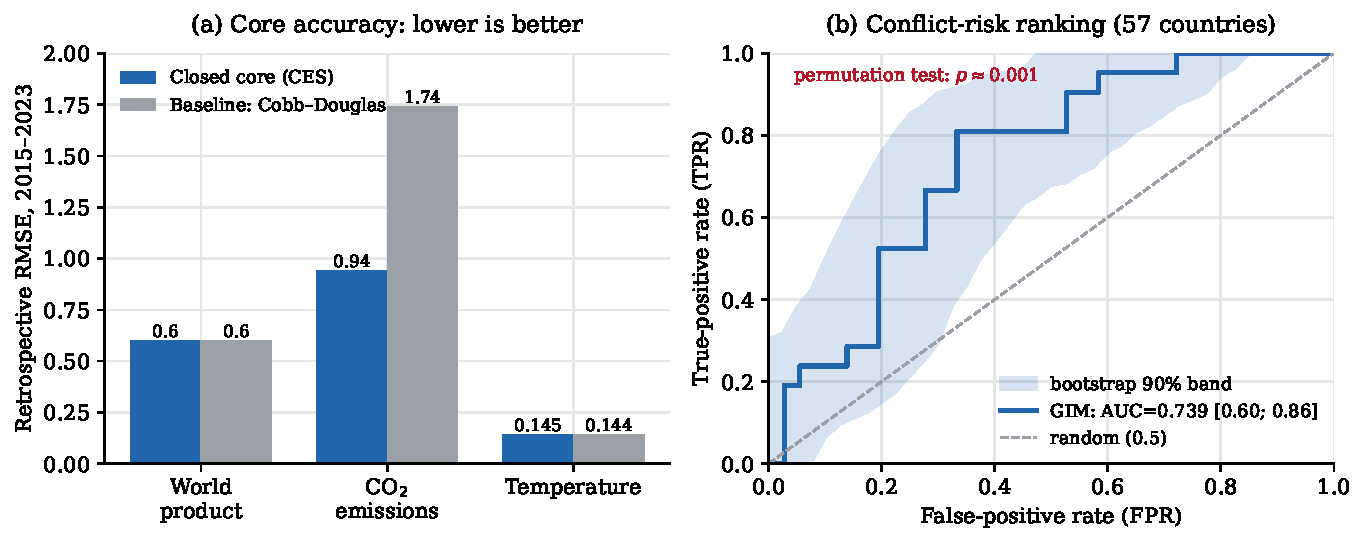
\includegraphics[width=\linewidth]{fig2_validation.pdf}
\caption{Retrospective anchor. \emph{(a)}~In-sample error 2015--2023. World product (T USD),
emissions (Gt) and temperature ($0.1\,^{\circ}$C) at left; the three resource prices at right,
scored as the ratio to the error a no-skill flat price makes, so the dashed line at unity is
that null and below it is better. \emph{(b)}~Conflict ranking against the benchmark that
decides it --- not chance, but the composite's own best single input. Bars are AUC with
$95\,\%$ bootstrap intervals; the paired difference and the probability that the composite is
the better ranker are inset (score inputs at 2023 base-year values; the vintage-clean variant
is given in the text).}
\label{fig:valid}
\end{figure}

\section{Does it do anything? Emergent dynamics}
\label{sec:emergent}

A simulator can be stable and anchored by being inert. The third requirement is that the loop
produce structured behaviour beyond the coded terms it builds on. We assess this regularity by
regularity, naming in each case the coded ingredient and the consequence that does not follow
from it directly.

\textbf{A lagged economy-to-society channel.} The coded ingredients are linear increments to an
accumulating tension index; the multi-year timescale itself follows from accumulation.
Identifying the channel requires care about which statistic is used, and the distinction is
general enough to state plainly: correlating priors with the terminal \emph{level} of an
accumulating variable recovers whichever coefficients set its drift, and drift coefficients are
coded terms. Only a paired shock-minus-baseline difference isolates the causal response, because
the drift cancels between the two arms. Here the two statistics disagree --- level and response
correlate at $r_s=-0.33$ across ensemble members, so the two questions have different
answers.

Read on the level, tension is governed by physico-economic priors, led by the base interest rate
($r_s=+0.40$) and equilibrium climate sensitivity ($r_s=+0.32$), with the social priors at
$|r_s|\approx0.2$. Read on the response, a three-year stagflation pulse raises mean tension to a
peak of $+0.0031$ five years later, positive in 82\,\% of prior draws at the peak, decaying back
toward zero by year ten ($+0.0002$): a hump rather than a ramp. Distributed-lag regression
confirms transmission at lag zero and at multi-year lags (cumulative effect $+0.33$,
within-$R^2$ $0.20$; Fig.~\ref{fig:social}). The prior governing that response is
\texttt{SOCIAL\_STRESS\_UNEMPLOYMENT\_SENS}, the coded economy-to-society coefficient, and the
largest single response loading is a climate-damage parameter ($r_s=-0.35$): the channel that
reaches society is physico-economic, and it is lagged. Global Morris screening over the 33 priors
\citep{morris1991,campolongo2007} is reported alongside. Throughout we give effect sizes rather
than $p$-values: on model-generated samples $p$ is a function of the run budget, not evidence
about the world. The spectrum of
Section~\ref{sec:stability} sees the same structure from the other side: its slow modes load on
trust and tension.

\textbf{Threshold-stepped sovereign cascades.} The staircase shape is coded --- thresholds
are thresholds. What is not coded is \emph{which} countries tip, in what order, and at what
dose: an oil-import burden propagates through reserves and debt issuance, leaving every importer
untouched at ${\approx}3\,\%$ of GDP, tipping three at $6\,\%$, four at $10\,\%$ and twelve at
$15\,\%$. The ordering follows each country's fiscal state --- pre-shock debt and reserves,
Spearman $-0.46$ and $-0.44$ against the tipping dose --- rather than any hand-set sequence, and
its dependence on two fiscal margins rather than one is what distinguishes it from a ranking on
the debt trigger's own variable (Appendix~\ref{app:benchmark}).

\textbf{Power-law escalation of food-driven instability.} The social increments are linear in
their inputs (Appendix~\ref{app:spec}), yet protest pressure responds to regional yield loss as a
power law with exponent ${\approx}1.1$ --- consistent in shape with the nonlinearity reported for
food prices and unrest by \citet{lagi2011food} (a working paper; we cite it as such). Where that
curvature originates matters, since composition across a block boundary and nonlinearity are
separate properties and the second does not follow from the first. Across a
sevenfold dose range the two legs of the chain carry nearly the same exponent ($1.17$ for
affordability stress, $1.09$ for protest pressure): the resource block generates the curvature and
the social block transmits it at a gain that varies only modestly with dose. The cross-block
composition is what brings the shock to society at all; it is not what makes the response
nonlinear.

\textbf{Cross-block synchrony of failures.} On the deterministic 30-year baseline active crises
rise from $5.9$ per year in the first decade to $14.4$ in the last. The natural summary of such a
rise is a dispersion index, and it is the wrong one: a Fano index computed on a trending
deterministic series measures the trend, so comparing it against the homogeneous-Poisson
reference of unity tests nothing. The appropriate reference is an \emph{inhomogeneous} Poisson
surrogate carrying the same fitted intensity, and against it the model shows no excess dispersion
at all --- surrogate mean $2.07$ against a model value of $1.39$, with residual dispersion about
a fitted trend of $0.51$, so the counts are in fact \emph{more} regular than Poisson. We note
this because dispersion indices are often quoted for trending simulated series, where without a
matched-intensity null they are uninformative.

The property that does hold is \emph{synchrony across blocks}. Onsets of economic crises
(sovereign debt, currency) and of social crises (regime) correlate at $+0.52$ at lag zero, with
centroids four years apart. Severing every cross-block channel --- the parameter set is given in
the repository --- halves that correlation to $+0.26$ while leaving the rise itself intact:
roughly half the co-timing is the coupling and half is each block's own clock. The ablation is
what makes this a measurement rather than an interpretation. The game layer shows
the same clock from the player's side: 77--90\,\% of losing runs fail after 2040
(Section~\ref{sec:instrument}).

\textbf{Spatially structured risk.} The diffusion itself is coded (neighbour spillover weight
$0.05$); what is measured is its effect. Switching it on costs under $0.01\,\%$ of the
2015--2023 retrospective fit, and it is not inert: switching the tension channel off raises the
cross-country dispersion of tension by $6.5\,\%$ and quadrupling the weight lowers it by
$2.2\,\%$, monotonically in the weight, while the crisis count moves by up to $21\,\%$ when the
whole spatial layer is removed. The \emph{climate}-risk diffusion, by contrast, has no
measurable downstream effect in the deterministic configuration. The reason is a limit of scope
rather than a defect: climate reaches society only through discrete
extreme events, which the deterministic runs switch off, leaving climate risk with only linear
consumers --- and a mean-preserving diffusion of a linear function changes nothing in aggregate.
With extreme events enabled over a seeded ensemble the same ablation does move tension and
crisis counts (by $1.7\,\%$ and $4.3\,\%$). A continuous climate-to-society term exists in the
code but ships disabled, because the literature that would set its magnitude is contested
(Section~\ref{sec:limits}). We do not claim that the emergent spatial autocorrelation matches
the observed record; that comparison lives in the repository's geographic validation materials.

\begin{figure}[t]
\centering
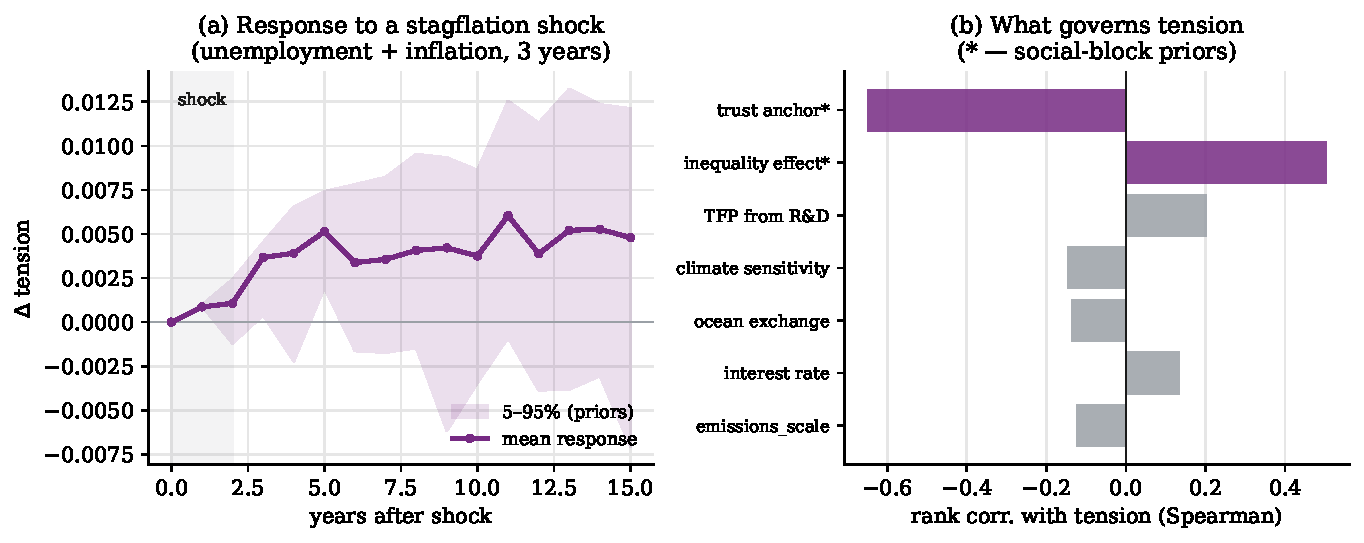
\includegraphics[width=\linewidth]{fig5_social_channel.pdf}
\caption{The economy-to-society channel. \emph{(a)}~Impulse response of mean tension to a
three-year stagflation shock: a hump peaking around year five and decaying by year ten (5--95th
band over priors). \emph{(b)}~What governs tension, contrasting the two questions: rank
correlation of each prior with the final tension \emph{level} and with the causal \emph{shock
response}. Social-block priors are marked~$*$. The level is led by physico-economic priors, and
the two statistics correlate at only $-0.33$ across members, which is why the claim rests on the
paired response in~(a) rather than on the level.}
\label{fig:social}
\end{figure}

\section{The instrument: ensembles, weak signals, and a game that hunts the tails}
\label{sec:instrument}

The model is operated as an instrument with three modes, in increasing order of adversarialness.

\textbf{Ensembles and scenario differences.} The core is deterministic, so uncertainty is
explicit: 500-member ensembles over the history-matched priors yield outcome distributions, and
scenarios are compared as distributions against a common baseline --- differences are robust to
the anchor uncertainties that dominate absolute levels. The whole workflow runs on a laptop
(Apple M4 Pro: a world-year in 30--50 ms, the 500$\times$30-year ensemble in under a minute,
the full 527-test suite in two), which is what makes ensemble-first practice a default rather
than a special exercise. A worked case: a \$50/tCO$_2$ carbon tax cuts emissions by
${\approx}5.5\,\%$ over ten years while raising tension and lowering trust through the
energy-price--inflation channel --- the political-economy cost invisible to single-domain
models, monotone in the rate, and directly relevant to observed reversals (France 2018,
Australia 2014); the full dose--response harness is Appendix~\ref{app:benchmark}.

\textbf{Weak signals.} Before any threshold fires, the joint state is monitored for early
structure: Mahalanobis distance of the stationary increments from their recent baseline
\citep{mahalanobis1936,wilson1931}, information-criterion change-point detection
\citep{schwarz1978}, and critical-slowing-down indicators \citep{scheffer2009}. On synthetic
and model trajectories an injected 15\,\% output drop is flagged at the correct step while calm
runs stay near the false-alarm rate; the working device is comparing a scenario's weak-signal
profile against the baseline's.

\textbf{The game as an adversarial tail sampler.} The same 57-actor core, wrapped into a
single-player decision game (GODMODE): thirty annual turns from 2023, a deck of 158 dilemma
cards compiled into real policy actions, seven catastrophe gates (temperature, biosphere,
stability, economic and geopolitical strain, energy and food prices); losing any gate ends the
run, reaching 2050 wins. A full game simulates in about a second, so outcome distributions are
statistically meaningful; and because players and scripted archetypes actively push the world
into corners smooth history never visits, the game functions as an importance sampler of the
tails. Three uses justify reporting it in a modeling paper.

\emph{A tail census.} In the 1,002-game reference batch of scripted archetypes, survival is
23.5\,\% with losses spread across five causes (35\,\% climate, 22\,\% economic, 21\,\%
geopolitical, 13\,\% stability, 8\,\% energy price) and 77\,\% of failures landing in
2040--2045 (Fig.~\ref{fig:game}). Production telemetry from the public deployment corroborates
the shape with humans in the loop: 401 runs were started by external players and 200 completed
(51\,\% attrition). Survival is $57/200 = 28.5\,\%$ of completers (95\,\% CI ${\pm}6.3$ points,
overlapping the best scripted archetype's $28.4\,\%$) but only $57/401 = 14.2\,\%$ of starts;
since abandonment plausibly correlates with a run going badly, the completer rate is an upper
bound. Human losses show a broader spectrum (31\,\% climate, 29\,\% economic, 15\,\%
geopolitical, plus biosphere, food, and energy tails the bots rarely hit), 90\,\% fall after
2040, and scores are bimodal (loss cluster near 26, win cluster 70--81, winners holding warming
to $1.6$--$1.9\,^{\circ}$C). The distribution of \emph{ways the world fails under active
management} is a model output no backtest can provide. Telemetry is anonymous by design and
reported only in aggregate (see Declarations).

\emph{Emergent strategy structure.} No doctrinaire policy dominates: uniformly random play
survives most often (28.4\,\%), beating consistent decarbonisation (20.1\,\%) and consistent
expansion (21.9\,\%), and each doctrine dies of its characteristic disease (green of economic
strain, 43\,\% of its losses; growth of climate and stability, 39\,\% and 34\,\%); passivity is
worst (18.7\,\%, two-thirds of losses to economic strain --- in a stock-flow-consistent world,
drifting means compounding debt). Restraint on both strain axes at once wins ${\approx}75\,\%$
against ${\approx}5\,\%$ for recklessness on both. Single-axis optimisation shifting the
binding constraint to another subsystem is the game-mechanical face of the coupling this paper
is about.

\emph{A diagnostic that found real defects.} Balancing the game exposed two structural
degeneracies: resource prices pinned at their clamps (a missing mean-reversion term plus two
compounding accounting defects), and government trust declining on hawk and dove paths alike
--- an attractor from an inequality drag ${\approx}40\times$ the only restoring term, the very
socio-fiscal subspace the spectrum of Section~\ref{sec:stability} flags. Neither was visible in
any 2015--2023 backtest; both fixes shipped as equilibrium anchors with the goldens
bit-identical (the trust anchor deliberately ships off in the headline configuration, so the
paper's stability numbers describe the conservative, weaker-anchored model). Sustained
adversarial play explores exactly the regions that validation against smooth history cannot; we
regard the game layer as part of the model's quality programme. (Its epistemic status is
bounded: the game provides no goodness-of-fit against history, human telemetry
reflects self-selected players with completion attrition, and difficulty gates are tuned
against the bot batches through threshold-flip analysis.)

Beyond the game, country policies can also be set by language-model agents (intentions
compiled into the same typed actions; every consequence computed by the deterministic core; off
in all validated configurations, with full prompt/response audit logs) --- the strategy space
widens without the physics ever leaving the engine. The whole environment --- CLI, ensembles,
games, a desktop analytical shell --- ships as an open, pip-installable codebase with pinned
goldens and dated, manifest-bound runs \citep{theclimateguy2026gim}; results here correspond to
release v18.1.3.

\begin{figure}[t]
\centering
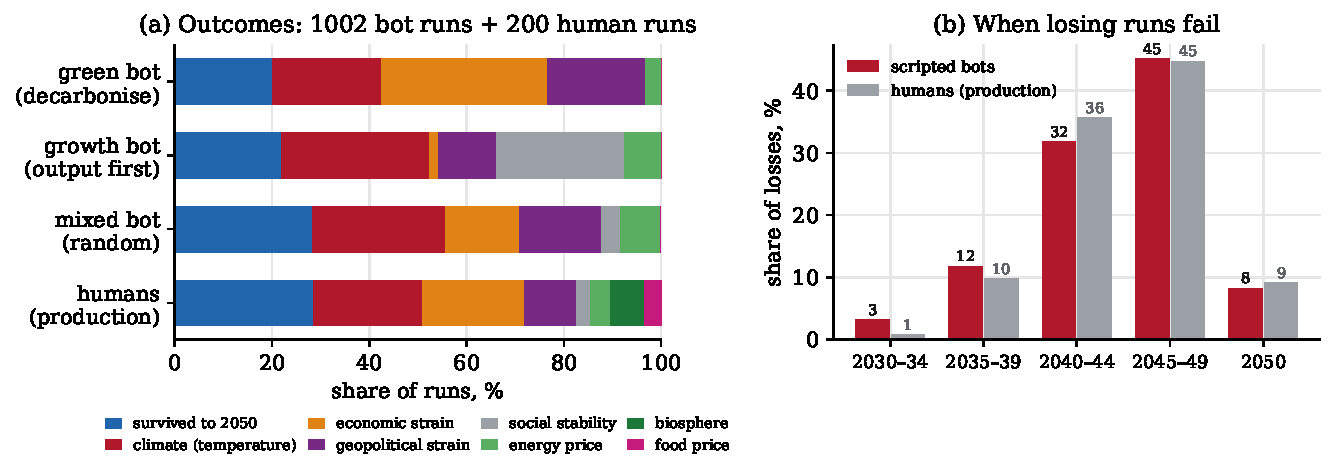
\includegraphics[width=\linewidth]{fig10_game_outcomes.pdf}
\caption{The tail census: 1,002 scripted playthroughs and 200 completed human runs (of 401
started; completer statistics shown, an upper bound under attrition), 2023--2050.
\emph{(a)}~Outcome composition by archetype and for human players: no doctrine dominates, each
dies of its characteristic cause, and the human loss spectrum is broader (biosphere and
food-price tails the bots rarely hit). \emph{(b)}~Timing of failures, bots vs.\ humans: both
distributions peak in 2040--2049 as slow accumulators come due.}
\label{fig:game}
\end{figure}

\section{Limitations}
\label{sec:limits}

\textbf{Convergence is engineered, not proven.} The anchors that stabilize the loop could mask
genuine instabilities of the real system; their strengths carry priors and the tails are probed
adversarially, but a formal stability proof for the full nonlinear map does not exist --- the
spectral and perturbation evidence of Section~\ref{sec:stability} is local and numerical. The
trust anchor is the clearest case of the trade-off: without it the model has a unit root in an
institutional variable and the spectral radius is set by that defect rather than by the coupling;
with it the model reverts toward each agent's base-year level, which is an assumption about the
world over a thirty-year horizon and not a neutral one.

\textbf{Resource prices reach the economy unevenly.} Forcing each price by a fixed multiple over
a ten-year run moves world output by $-5.5\,\%$ (energy), $-7.9\,\%$ (food) and $+0.8\,\%$
(metals) at a fivefold shock. The metals price is close to inert downstream. Food reaches society
mainly through the trade balance and the sovereign channel rather than through consumer prices,
and the food cost-push term into inflation was added only in this version.

\textbf{Climate reaches society only through discrete events.} There is no continuous
climate-to-tension term in the headline configuration. One exists in the code, disabled: the
canonical prior for it \citep{hsiang2013} reports a $14\,\%$ rise in intergroup conflict per
standard deviation of warming, but that meta-analysis is contested on sample selection and
analytical coherence \citep{buhaug2014}, with a reply disputing the reanalysis. The direction is
defensible and the magnitude is not identified, so we ship the mechanism off and tagged rather
than choosing a number, and every result in this paper is produced with it disabled.

\textbf{Crop response to warming is newly endogenous and rests on two priors.} Before this
version warming did not affect crops at all. It now does, at the per-degree yield losses of
\citet{zhao2017}, composed with an agricultural supply price elasticity \citep{haile2016}; the
first excludes adaptation and the second supplies it. Taken alone either is misleading --- the
yield channel without a supply response drives the food price to its ceiling. The pair gives a
$+24\,\%$ food price by 2053, inside the range assessed by the IPCC for climate-driven cereal
prices at 2050, an anchor it was not fitted to.

\textbf{Expectations are adaptive.} Agents look at the recent past; a tested model-consistent
expectations mechanism is off by default (its marginal effect proved unstable). Anticipatory
responses to announced policy are not in the headline runs.

\textbf{Long-run growth is weakly identified,} and forward projections anchor productivity
drift to an external scenario; absolute long-horizon levels inherit this, which is why scenario
differences are the recommended mode.

\textbf{The climate block is a fast emulator,} not an Earth-system model; the strongest carbon
feedbacks are deeply uncertain, switchable, and relegated to tail scenarios. Damage estimates
are uncertain across the discipline and carried as an interval (the level function is anchored
at the meta-analytic central estimate; a Burke-type growth-damage channel exists as a switch).

\textbf{The socio-political block mixes anchored and expert-set pieces.} Substantial parts are
tied to literature (war-size tail, migration gravity, misery-index ratio, governance anchors);
coupling thresholds and cross-border tension diffusion remain expert priors, tagged as such in
the auditable registry. Conflict is intrinsically hard to predict: the block supports relative
risk ranking (AUC ${\approx}0.74$; vintage-clean 0.84), not event prediction. The persistent
social mode found in Section~\ref{sec:stability} means socio-political initial-state errors do
not wash out --- an inherited uncertainty, and a larger one than the economic case. Statistics
computed on ensemble output (Section~\ref{sec:emergent}) identify internal channels, not
external facts, and are reported as effect sizes for that reason.

\textbf{No nominal exchange rate, and the currency channel depends on that.} The currency-crisis
mechanism now fires at a rate and duration consistent with the observed record ($3.5\,\%$ of
eligible agent-years against $3$--$5\,\%$; mean duration $1.9$ years against $1$--$3$), but only
because the episode length is bounded explicitly. Nothing in the model rebuilds reserves, since
there is no depreciation to compress imports, so a reserve-accumulation identity is implemented
and deliberately left disabled: switching it on drives the crisis rate to $8\,\%$. Agents that do
not issue their own currency or that issue a reserve currency are exempt from the trigger by an
explicit list, because the model carries no monetary-union concept and would otherwise flag
euro-area members --- as it did, until the historical backtest caught it.

\textbf{Aggregation.} Resources are aggregate (no sectoral energy technologies, no endogenous
renewable learning curves); no portfolio capital account; no dedicated
pandemic submodel (epidemic shocks are extreme events); state-dominated political economies are
represented by shared functional forms with country-specific states.

\section{Conclusion}

The contribution of this work, restated in its proper order: a closed seven-domain,
57-agent world simulator that (i)~stays together --- a spectral radius near unity whose
above-unity modes are now mainly economic and whose climate subspace contracts entirely, with
contracting economic and climate perturbations and near-linear uncertainty growth over thirty
years; (ii)~is anchored --- in-sample and free-running out-of-sample retrospective evaluation
across output, emissions, temperature and resource prices, external cross-checks, an
input-vintage-robust conflict ranking reported against its own best single covariate; and
(iii)~is responsive --- a lagged social impulse response, threshold cascades, power-law
escalations, and failures that synchronize across blocks more than the blocks alone would
produce. Underneath is a stated philosophy: the
deterministic core encodes explicit invariants of nature and society --- conservation,
accounting, slow empirical regularities --- with calibrated restoring forces, and all
uncertainty lives in ensembles over the invariants' strengths. Around it is an instrument:
history-matched ensembles for distributions, weak-signal detectors for early structure, and a
game layer that adversarially samples the tails, yields outcome distributions from both
scripted archetypes and external human players, and has already paid for itself by exposing two
structural degeneracies that no retrospective test could see. The model does not forecast; it
maps the consequences of assumptions, the distribution of risks, and the ways a managed world
can fail --- comparatively, reproducibly, and on a laptop.

\section*{Declarations}

\textbf{Ethics and player telemetry.} The game telemetry reported in
Section~\ref{sec:instrument} is anonymous by design and analysed only in aggregate. The public
deployment records, per run: a randomly generated run identifier, the random seed, the in-game
outcome (win/loss, cause, year), the composite score, and final in-game aggregate metrics.
There are no accounts; no names, e-mail addresses, IP addresses, demographic attributes, or
device identifiers are collected or stored with runs; an optional nickname may be submitted
after a run for the public leaderboard and is excluded from the analysis here. On this basis
the collection was judged to fall outside the scope of human-subjects review (non-interventional,
anonymous gameplay statistics); no ethics approval was therefore sought, and no individual-level
data are reported.

\textbf{Conflict of interest.} N.S.S. and A.A.O. are employees of JSC Sberbank of Russia, whose
risk-management activities are adjacent to the model's stated use cases; the bank had no role in
study design, analysis, or the decision to publish. The authors declare no other competing
interests.

\textbf{Funding.} This research received no funding of any kind and was carried out entirely on
the authors' own time; article processing charges are borne by the authors.

\textbf{Author contributions (CRediT).} N.S.S.: conceptualization, methodology, software (the
simulation engine and the game layer), investigation, writing --- original draft. A.A.O.:
validation (model validation programme), writing --- original draft and review \& editing.
A.N.K.: validation (model and game-simulator testing), formal analysis (assessment of results),
writing --- review \& editing. The archived software is authored by N.S.S. and A.A.O.; the
Zenodo deposit's author list reflects the software, the byline reflects the paper.

\textbf{Generative-AI disclosure.} Large-language-model tools were used as coding and
manuscript-editing assistants (drafting support, reference formatting, and consistency checks);
all analyses, results, and claims were produced by the deterministic model harnesses and
verified by the authors, who take full responsibility for the content. LLM use \emph{inside}
the model is a documented, optional feature (Section~\ref{sec:instrument}) and is off in every
validated configuration.

\section*{Code and data availability}
The complete model, calibration data with checksums, every validation and stability harness
cited in the text, the game backend, and the figure-generation scripts are openly available at
\url{https://github.com/Theclimateguy/GIM} \citep{theclimateguy2026gim}; the archived Zenodo
deposit is version 18.1.4 (\url{https://doi.org/10.5281/zenodo.21575176}), an archival
repackaging of the v18.1.3 engine with no code change --- all results in this paper correspond
to that engine and are reproducible on a consumer laptop from the pinned release.

\clearpage
\appendix
\section{Model specification and key parameters}
\label{app:spec}

\textbf{Production.} Output is nested CES in capital, labour, and energy, normalized to
Cobb--Douglas at each country's base point \citep{arrow1961}:
\begin{equation}
Y = A\,\Theta\,\mathrm{KE}_0^{\,\alpha+\gamma}\big(a_K (K/K_0)^{\rho_{KE}} + a_E (E/E_0)^{\rho_{KE}}\big)^{(\alpha+\gamma)/\rho_{KE}} L^{\beta},
\qquad \rho_{KE} = \tfrac{\sigma_{KE}-1}{\sigma_{KE}},
\label{eq:ces}
\end{equation}
with $\alpha=0.30$, $\beta=0.60$, $\gamma=0.042$, $a_K=\alpha/(\alpha+\gamma)$,
$a_E=\gamma/(\alpha+\gamma)$, $\mathrm{KE}_0=K_0^{a_K}E_0^{a_E}$; at the base point the inner
aggregator (the parenthesis) equals one because $a_K+a_E=1$, so levels and first derivatives
reproduce the Cobb--Douglas limit for any $\sigma_{KE}$, while substitution away from it is
governed by $\sigma_{KE}=0.4$ (gross complementarity \cite{vanderwerf2008,koetse2008};
factor shares from the Penn World Table \cite{feenstra2015,gollin2002}). The exponent sum $0.942$ encodes mild
decreasing returns; per-country scale factors pin base-year levels, so renormalising to
constant returns moves 2100 world product by only 7--9\,\%. Capital:
$K_{t+1}=(1-\delta)K_t+sY_t$, $\delta=0.05$, $s\approx0.24$ modulated by stability and tension
\citep{mody2012}. Productivity grows at ${\approx}1\,\%$ baseline with R\&D
(\`a la Jones \cite{jones1995}), trade diffusion, and $\beta$-convergence (slope 0.0093 per
log gap, validated on the cross-section); inflation is Phillips-with-pass-through plus a weak
quantity-theory term ($\lambda\approx0.027$); rates follow country Taylor rules capped
$\pm6$\,pp \citep{taylor1993}.

\textbf{Climate.} Four-pool AR6 impulse response \citep{joos2013}:
\begin{equation}
C^{(i)}_{t+1} = C^{(i)}_t e^{-1/\tau_i} + a_i E_t,\quad
a=(0.2173,0.2240,0.2824,0.2763),\ \tau=(\infty,394,36.5,4.3)\,\text{yr},
\label{eq:pools}
\end{equation}
(shares sum to one exactly; rounded here). Forcing is
$F=5.35\ln(C/C_0)+F_{\text{non-CO}_2}$ --- the \citet{myhre1998} coefficient, implying
$F_{2\times}=3.71$~W\,m$^{-2}$ and, at the calibrated equilibrium sensitivity of
$3.0\,^{\circ}$C, a feedback parameter $\lambda=1.24$~W\,m$^{-2}$K$^{-1}$; the AR6-updated
$F_{2\times}$ is higher, but since sensitivity is calibrated at doubling the equilibrium anchor
is unaffected and the transient response is checked directly (TCR $1.79\,^{\circ}$C, within the
AR6 likely range) --- with the non-CO$_2$ term on the SSP2-4.5 marker forward. Two-layer heat
balance \citep{geoffroy2013}:
\begin{equation}
C_s\dot T = F - \lambda T - \kappa(T-T_d), \qquad C_d\dot T_d = \kappa(T-T_d).
\label{eq:ebm}
\end{equation}
Damage: $\Omega(T)=1-0.0078\,T^2$ (3.1/7.0/12.5\,\% at $+2/+3/+4\,^{\circ}$C), anchored at the
Howard--Sterner productivity-corrected central estimate \citep{howard2017,nordhaus2017},
normalized to the 2023 baseline; Burke-type growth damages switchable
\citep{burke2015,burke2023}.

\textbf{Society and crises.} Tension is a $[0,1]$ composite (base year: WGI-derived trust and
stability, Gini, water stress, climate risk; increments: unemployment $0.010$/pt, inflation
$0.005$/pt, inequality damped by individualism, trust anchor, neighbour spillover $0.05$).
Legitimacy $=0.6\,\text{trust}+0.4(1-\text{tension})$ sets the policy-space multiplier. Crisis
triggers (expert priors, tagged in the registry): debt --- debt${}>120\,\%$ GDP and effective
rate${}>12\,\%$ (then a 40\,\% write-down, 7\,\% output loss, exit below 70\,\%/8\,\% within 6
years); currency --- external debt${}>50\,\%$, current-account deficit${}>4\,\%$, reserves
${}<3$ months; regime collapse --- trust${}<0.20$ and tension${}>0.80$. Severity optionally
heavy-tailed (war-size exponent $\alpha_w\approx1.5$ \cite{richardson1948,clauset2009}).

\begin{table}[h]
\centering
\small
\caption{Key priors, part 1: the 19 parameters discussed in the text (units inline; dimensionless
unless stated). Central values and 5--95th plausibility ranges.}
\label{tab:priors1}
\begin{tabularx}{\linewidth}{@{}lccL@{}}
\toprule
Parameter & Central & Range & Source \\
\midrule
Equilibrium climate sensitivity, $^{\circ}$C & 3.0 & 1.5--6.0 & \citep{ipcc_ar6_wg1,otto2013} \\
Surface heat capacity, W\,yr\,m$^{-2}$K$^{-1}$ & 8.0 & 6.0--18.0 & \citep{geoffroy2013} \\
Ocean heat exchange, W\,m$^{-2}$K$^{-1}$ & 1.0 & 0.4--1.3 & \citep{geoffroy2013} \\
Emissions scale & 0.98 & 0.90--1.05 & \citep{friedlingstein2023} \\
Structural decarbonization rate, yr$^{-1}$ & 0.016 & 0.010--0.030 & GCP/WDI trend \citep{friedlingstein2023}; 2015--2023 backtest \\
Capital share $\alpha$ & 0.30 & 0.22--0.40 & \citep{feenstra2015,gollin2002} \\
Labor share $\beta$ & 0.60 & 0.50--0.72 & \citep{feenstra2015,gollin2002} \\
Energy elasticity $\gamma$ & 0.042 & 0.015--0.080 & 2015--2023 backtest \\
Capital--energy substitution $\sigma_{KE}$ & 0.40 & 0.20--0.60 & \citep{vanderwerf2008,koetse2008} \\
Depreciation rate $\delta$, yr$^{-1}$ & 0.05 & 0.03--0.08 & \citep{feenstra2015} \\
TFP sensitivity to R\&D & 0.30 & 0.10--0.60 & calibration to backtest \\
Damage coefficient & 0.0078 & 0.0015--0.025 & \citep{howard2017,nordhaus2017,burke2015} \\
Pure time preference & 0.015 & 0.001--0.030 & \citep{nordhaus2017,stern2007} \\
Elasticity of marginal utility $\eta$ & 1.45 & 1.0--2.0 & \citep{nordhaus2017,stern2007} \\
Market demand elasticity & 0.40 & 0.20--0.70 & \citep{labandeira2017} \\
\midrule
\multicolumn{4}{@{}l}{\emph{Social block (validated by sign and channel, Sec.~\ref{sec:emergent})}}\\
Tension stress from unemployment & 0.010 & 0.007--0.014 & \citep{ditella2001}; structural prior \\
Tension stress from inflation & 0.005 & 0.003--0.007 & \citep{ditella2001} (aversion ${\approx}$2:1); prior \\
Inequality effect on tension & 0.0005 & 0.0003--0.0007 & \citep{wilkinson2009} \\
Trust-anchor strength & 0.060 & 0.039--0.081 & calibrated to WGI trust persistence \\
Trust mean-reversion pull, yr$^{-1}$ & 0.10 & 0--0.20 & weakest value lowering $\rho$ at all three linearization points (Sec.~\ref{sec:stability}) \\
\midrule
\multicolumn{4}{@{}l}{\emph{Resource block}}\\
Energy demand income elasticity & 0.50 & 0.33--0.60 & IEA intensity trend vs.\ world GDP growth \\
Food yield loss per $^{\circ}$C & 0.049 & 0.031--0.074 & \citep{zhao2017}, four independent method families \\
Food supply price elasticity & 0.143 & 0.045--0.79 & \citep{haile2016}, aggregate long-run growing area \\
Food price pass-through to CPI & 0.04 & 0.02--0.08 & CPI food weight $\times$ commodity-to-retail pass-through \\
\bottomrule
\end{tabularx}
\end{table}

\begin{table}[h]
\centering
\small
\caption{Key priors, part 2: the remaining 14 of the 33 sampled parameters (all switch-off
mechanisms sampled only in tail scenarios are excluded from headline runs).}
\label{tab:priors2}
\begin{tabularx}{\linewidth}{@{}lccL@{}}
\toprule
Parameter & Central & Range & Source \\
\midrule
Warming-benefit cap & 0 & 0--0.02 & prior (CO$_2$ fertilisation; off headline) \\
Warming-benefit peak, $^{\circ}$C & 0.3 & 0--1.0 & prior (deprecated; inactive while the cap is 0) \\
Damage risk adjustment & 0.005 & 0--0.02 & prior \\
Deep-ocean heat capacity & 100 & 40--200 & Geoffroy et al.\ 2013; DICE-2016 \\
Land-use CO$_2$, Gt/yr & 0.6 & 0--1.5 & Global Carbon Project 2023 \\
Carbon feedback, GtCO$_2$/$^{\circ}$C & 1.5 & 0--5.0 & AR6 WG1 Ch.5; permafrost literature \\
CH$_4$ feedback, W\,m$^{-2}$/$^{\circ}$C & 0.03 & 0--0.1 & AR6 WG1 Ch.5 (prior central; set to 0 in headline runs) \\
Base birth rate & 0.025 & 0.015--0.035 & World Bank WDI \\
Base death rate & 0.012 & 0.007--0.017 & World Bank WDI \\
Neutral interest rate & 0.02 & 0.005--0.04 & IMF WEO; $r^*$ literature \\
Growth-damage TFP coefficient & 0 & 0--0.001 & Burke et al.\ 2015 (off headline) \\
War-size tail exponent $\alpha_w$ & 1.5 & 1.3--1.8 & \citep{richardson1948,clauset2009} \\
Migration base / max share & 0.001/0.003 & see registry & UN DESA; UNHCR \\
Regime-collapse output/capital mult. & 0.8/0.7 & 0.7--0.9 / 0.55--0.85 & Barro \& Urs{\'u}a 2008 \\
\bottomrule
\end{tabularx}
\end{table}

\textbf{History matching and ensemble formation.} Priors are per-parameter triangular (30 of
33), lognormal (2), or normal (1) distributions with the ranges of
Tables~\ref{tab:priors1}--\ref{tab:priors2} (full registry in the repository). Implausibility
uses tolerances $\mathrm{tol}_o$ of $6$ trillion USD (world product), $2$ Gt (emissions), and
$0.15\,^{\circ}$C (temperature) --- observational uncertainty bundled with an explicit
model-discrepancy allowance --- with the cut $\max_o I_o \le 3$. The published configuration
uses a single wave of $60$ Latin-style random draws over the six backtest-driving parameters;
at the three-sigma cut the acceptance rate is $100\,\%$ (the cut removes only corners more
implausible than three combined standard errors, and the priors are already
literature-bounded), so the NROY region coincides with the prior box and ensembles draw all 33
parameters independently from their priors. This is disclosed rather than hidden: the
tolerances are wide because model discrepancy dominates, and tighter waves are future work.
The 33 key parameters carry literature-grounded priors; the full registry of 287 parameters
with calibration-status tags, all data-source manifests, and every harness cited in the text
are in the repository \citep{theclimateguy2026gim}.

\clearpage
\section{Integration benchmark: where sectoral models stop}
\label{app:benchmark}

For three shocks we take a published conclusion from a named sectoral model, feed GIM the same
exogenous shock, and ask whether it (a)~reproduces the sectoral first-order effect and
(b)~surfaces a cross-sector consequence the sectoral model cannot represent by construction.
Runs are deterministic (57 countries, ten years, extreme events off), and each scenario carries a
dose--response sweep.

We characterize each channel by the \emph{shape and gain} of its transfer function. Reporting a
nonzero GIM slope against the sectoral anchor's flat one would not be a measurement: a model
without a society block has zero slope on the society axis by construction. The sectoral
comparison establishes that GIM reproduces the first-order effect; the sweeps establish the form
of the cross-sector response, and the three forms differ.

\emph{Carbon tax (anchor: DICE \cite{nordhaus2017}).} Fed the same \$50/tCO$_2$ tax, GIM
reproduces the emissions decline (${\approx}5.5\,\%$ over ten years, log-log exponent $0.90$ in
the tax rate --- mildly saturating) and adds the political-economy channel: tension rises and
trust falls in the rate, with exponent ${\approx}1.8$.

\emph{Oil shock (anchor: energy-system models).} An oil-import burden propagates into sovereign
finance through reserves and debt issuance. The response is threshold-stepped: no importer tips
at $3\,\%$ of GDP per year, three tip at $6\,\%$, four at $10\,\%$, twelve at $15\,\%$ and
nineteen at $20\,\%$ (Sri Lanka 2022 is the real-world instance of the mechanism). Two features
of the construction bear stating. The supply cut is converted into an import bill \emph{outside}
the model, using an assumed price elasticity and import intensity, and injected into debt and
reserves, so the scenario exercises the finance-to-crisis leg rather than the
resources-to-finance one. And the tipping order depends jointly on pre-shock debt and reserves
(Spearman $-0.46$ and $-0.44$ against the tipping dose); that it turns on two fiscal margins
rather than one is what distinguishes it from a ranking on the debt trigger's own variable.

\emph{Crop shock (anchor: AgMIP/AR6).} A regional yield loss raises food-affordability stress and
protest pressure as power laws of similar exponent ($1.17$ and $1.09$) \citep{lagi2011food}: the
curvature is generated in the resource block and transmitted to society at a gain that varies
only modestly with dose (Section~\ref{sec:emergent}). The assessment chain stops at the
food-security index.

The three channels take distinct forms --- power-law, threshold-stepped, and power-law with a
different exponent (Fig.~\ref{fig:bench-summary}) --- and that variety, rather than a nonzero
slope, is what the benchmark establishes.

\begin{figure}[t]
\centering
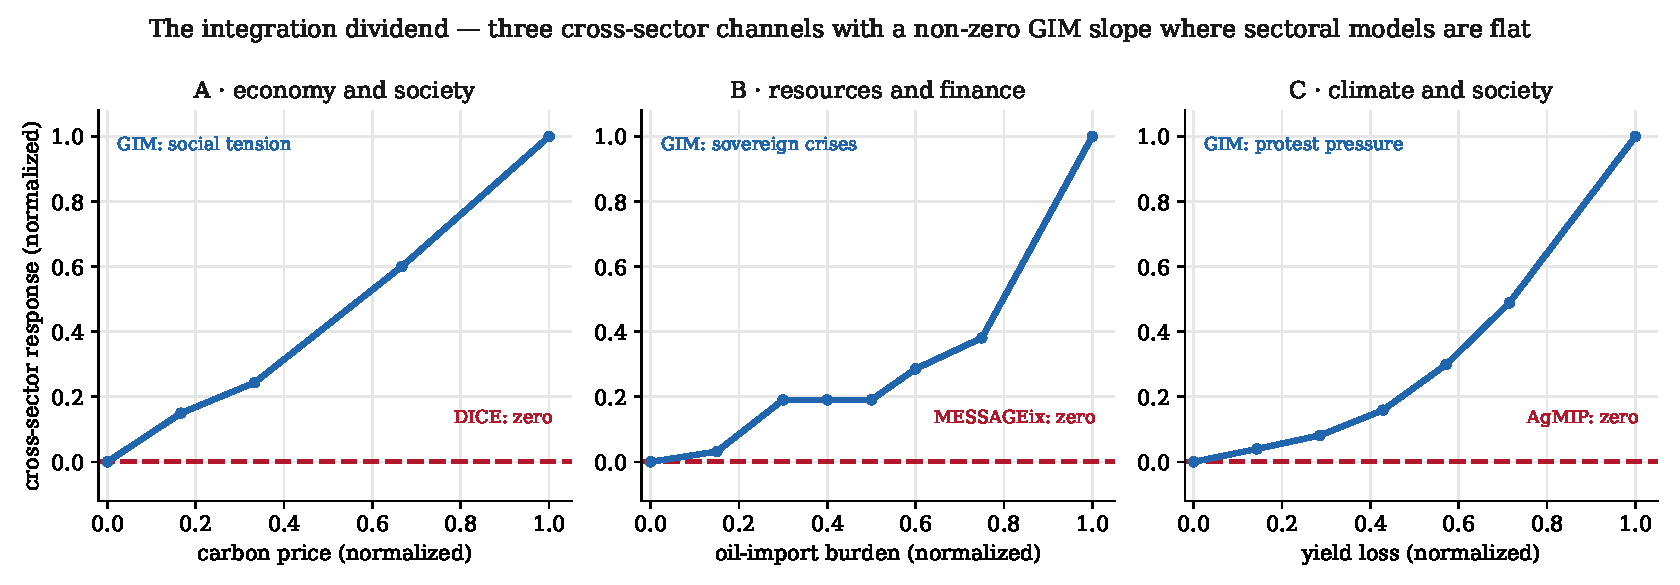
\includegraphics[width=\linewidth]{fig9_integration_summary.pdf}
\caption{Three cross-sector transfer functions, each in its own units.
\emph{(a)}~Carbon price to social tension: a power law, exponent $1.8$.
\emph{(b)}~Oil-import burden to the count of importers entering sovereign debt crisis:
threshold-stepped, six distinct levels, no importer tipping below $6\,\%$ of GDP per year.
\emph{(c)}~Regional yield loss to food affordability (grey) and protest pressure (green):
power laws of similar exponent, $1.17$ and $1.09$, so the curvature is generated in the
resource block and transmitted rather than compounded.}
\label{fig:bench-summary}
\end{figure}

\clearpage
\bibliographystyle{unsrtnat}
\bibliography{references_v2}

\end{document}
